\section{Results}
\label{sec:results}

\subsection{RQ1: OBTF Forecasts versus \mbox{ENTSO-E} Forecasts}
\label{sec:results_rq1}

Table~\ref{tab:rq1_component_forecast_results} compares OBTF
forecasts with the corresponding \mbox{ENTSO-E} day-ahead forecasts, each
evaluated against the same realized value. For load, the OBTF forecast is
the forecast-correction model of Section~\ref{sec:load_model}, created at the
final pre-gate-closure run before 12:00, so the comparison is against the
uncorrected \mbox{ENTSO-E} load forecast that this model takes as its baseline. The direct OBTF load model, which
uses no \mbox{ENTSO-E} forecast, is not part of the fixed comparison in
Table~\ref{tab:rq1_component_forecast_results}, but is benchmarked against
\mbox{ENTSO-E} separately below and enters RQ3 at cutoff times before the public
\mbox{ENTSO-E} load forecast is available. For solar and wind, the
\mbox{ENTSO-E} benchmark forecast is missing for a small number of timestamps,
which are dropped from the matched panel.

\begin{table}[htbp]
  \centering
  \small
  \setlength{\tabcolsep}{4.2pt}
  \caption[Accuracy of the OBTF load, solar, and wind forecasts versus \mbox{ENTSO-E}.]
  {Accuracy of OBTF load, solar, and wind forecasts compared with
  \mbox{ENTSO-E} forecasts.}
  \label{tab:rq1_component_forecast_results}
  \begin{threeparttable}
  \begin{tabular}{@{}lrrrrrrr@{}}
    \toprule
    Target & \(n\) & \multicolumn{2}{c}{RMSE} &
    \(\Delta\) RMSE\tnote{a} & \multicolumn{2}{c}{MAE} &
    \(p_{\mathrm{GW}}\)\tnote{b} \\
    \cmidrule(lr){3-4} \cmidrule(l){6-7}
    & & OBTF & \mbox{ENTSO-E} & & OBTF & \mbox{ENTSO-E}
    \\
    \midrule
    Load & 17,376 & \textbf{1,727} & 2,697 & \textbf{-36.0\%}
      & \textbf{1,350} & 2,140 & \(<0.001\) \\
    Solar gen. & 17,280 & 2,301 & \textbf{1,370} & +68.0\%
      & 1,109 & \textbf{747} & \(<0.001\) \\
    Wind gen. & 17,184 & 3,119 & \textbf{2,248} & +38.8\%
      & 2,092 & \textbf{1,450} & \(<0.001\) \\
    \bottomrule
  \end{tabular}
  \begin{tablenotes}[flushleft]
    \footnotesize
    \item[a] \(\Delta\) RMSE is computed relative to the corresponding
    \mbox{ENTSO-E} forecast. Negative values indicate lower errors of the OBTF forecast. All error values are in MW. The column \(n\) gives the
    number of matched observations used for the comparison. The evaluation
    window is 1~February~2026 to 31~July~2026. The renewable-generation
    comparisons have fewer observations because the \mbox{ENTSO-E} solar and
    wind benchmark forecasts are missing for some timestamps, and the wind
    comparison excludes 7~February~2026, for which no \mbox{ICON-D2} run with
    wind fields is archived.
    \item[b] One-sided GW p-value for the forecast with the lower
    RMSE against the alternative forecast, using paired squared-error loss
    differences.
  \end{tablenotes}
  \end{threeparttable}
\end{table}

The load result supports the first part of
\hyperlink{hyp:component_forecast_quality}{H1}. The OBTF load forecast
reduces the RMSE from 2,697~MW to 1,727~MW, a 36.0\%
error reduction relative to the \mbox{ENTSO-E} load forecast, with a comparable
reduction in MAE. This pattern is
consistent with the model design, because the OBTF load forecast used here corrects the public \mbox{ENTSO-E} forecast instead
of replacing it with an independent direct forecast. It can therefore combine
the public forecast with recent morning load and weather information available
before gate closure. Because the two forecasts do not share an information
cutoff, this is an operational rather than a like-for-like modeling comparison:
the \mbox{ENTSO-E} forecast is produced by an undisclosed model and issued at a
generally earlier, unspecified time, so the 36.0\% reduction measures the
operational value of the additional pre-gate-closure information the correction
exploits rather than a difference in modeling skill alone. A stricter comparison
nonetheless isolates a genuine modeling component: the direct OBTF load model, which
uses only open data and does not use the \mbox{ENTSO-E} forecast at all, still
reduces RMSE by 17.3\% relative to \mbox{ENTSO-E} when it is formed at the 10:30
cutoff at which the public forecast is published, a difference that is
statistically significant (GW p-value of 0.003). Correcting the
public forecast then extends this advantage to 36.0\%. Within this
operational setting, the OBTF load forecast is not only
competitive with the \mbox{ENTSO-E} forecast, but substantially more accurate in this
test window. The GW test supports this ranking with a p-value
below 0.001.

The renewable-generation comparison shows the opposite pattern. The OBTF solar forecast
has an RMSE of 2,301~MW compared with 1,370~MW for the \mbox{ENTSO-E} solar
forecast. The OBTF wind forecast has an RMSE of 3,119~MW compared with
2,248~MW for the \mbox{ENTSO-E} wind forecast. The \mbox{ENTSO-E}
renewable-generation forecasts therefore outperform the OBTF solar and
wind forecasts in this benchmark comparison. The GW test also
supports the \mbox{ENTSO-E} ranking for both renewable-generation targets. For
solar and wind, however, the \mbox{ENTSO-E} forecasts are not admissible inputs
for the operational price forecast studied in this thesis. The \mbox{ENTSO-E}
forecasts used here are not publicly observable before the 12:00
day-ahead gate closure, while the OBTF solar and wind forecasts are restricted
to information that is available before gate closure. The higher errors of the OBTF solar and wind
forecasts therefore do not rule out their relevance for the price model.

Overall, \hyperlink{hyp:component_forecast_quality}{H1} is supported. The
OBTF load forecast is not only competitive with but more accurate than
the \mbox{ENTSO-E} forecast, and the OBTF solar and wind forecasts have
higher errors than the \mbox{ENTSO-E} benchmarks, as expected. The renewable gap
is substantial, however, with an RMSE that is 68.0\% higher for solar and 38.8\%
higher for wind. The
result therefore establishes the empirical trade-off for RQ2: the OBTF solar and wind forecasts are less accurate than their
\mbox{ENTSO-E} benchmarks, but they are admissible inputs for the
price forecast. Whether this operationally available
representation still improves the price forecast is tested in RQ2.

\subsection{RQ2: Explicit Load and Renewable-Generation Forecasts in Price Forecasting}
\label{sec:results_rq2}

\hyperlink{rq:price_impact_generated_forecasts}{RQ2} tests how an explicit
representation of load and renewable-generation forecasts affects the
day-ahead price forecast.
This representation consists of the OBTF load forecast, the
OBTF combined renewable-generation forecast, and the OBTF
residual-load forecast.
Table~\ref{tab:rq2_price_results} reports the
out-of-sample accuracy of the two naive benchmarks and the three price
forecasts from the boosted-tree price model, all evaluated on the same matched panel of delivery days and
MTUs.

\begin{table}[htbp]
  \centering
  \small
  \setlength{\tabcolsep}{5.5pt}
  \caption[Price forecast accuracy with and without OBTF forecasts.]
  {Out-of-sample price forecast accuracy of the naive benchmarks and the
  price forecasts with and without OBTF load and renewable-generation forecasts.}
  \label{tab:rq2_price_results}
  \begin{threeparttable}
  \begin{tabular}{@{}lrrrrr@{}}
    \toprule
    Forecast & \(n\) & RMSE & \(\Delta\)RMSE\tnote{a} & MAE
      & \(p_{\mathrm{GW}}\)\tnote{b} \\
    \midrule
    \(\mathrm{N}_{d-1}\)
      & 17,184 & 49.69 & +40.0\% & 30.63 & \(<0.001\) \\
    \(\mathrm{N}_{d-7}\)
      & 17,184 & 60.31 & +69.9\% & 38.18 & \(<0.001\) \\
    \(\hat{P}^{\mathrm{base}}\)
      & 17,184 & 35.50 & --- & 20.82 & --- \\
    \(\hat{P}^{\mathrm{gen}}\)
      & 17,184 & \textbf{31.54} & \textbf{-11.2\%} & \textbf{18.05} & \(<0.001\) \\
    \(\hat{P}^{\mathrm{gen},-\mathrm{wea}}\)
      & 17,184 & 31.79 & -10.5\% & 18.18 & \(<0.001\) \\
    \bottomrule
  \end{tabular}
  \begin{tablenotes}[flushleft]
    \footnotesize
    \item[a] \(\Delta\)RMSE is computed relative to
    \(\hat{P}^{\mathrm{base}}\). Negative values indicate lower errors
    than the base price forecast. All error values are in EUR/MWh. The column
    \(n\) gives the number of matched observations. The evaluation window is
    1~February~2026 to 31~July~2026, with 7~February~2026 (no archived wind
    input) and 19~June~2026 (weather input unavailable) removed.
    \item[b] One-sided GW p-value between the row forecast and
    \(\hat{P}^{\mathrm{base}}\), for the forecast with the lower RMSE of
    the two, using paired squared-error loss differences.
  \end{tablenotes}
  \end{threeparttable}
\end{table}

Explicitly representing load and renewable generation improves the price
forecast. The price forecast with OBTF load and renewable-generation forecasts,
\(\hat{P}^{\mathrm{gen}}\), reduces the RMSE from
35.50~EUR/MWh for the base forecast
\(\hat{P}^{\mathrm{base}}\) to 31.54~EUR/MWh, a
reduction of 11.2\%, with a comparable reduction in MAE. The
GW test rejects equal predictive accuracy in favor of
\(\hat{P}^{\mathrm{gen}}\), with a p-value below 0.001.
\hyperlink{hyp:price_impact_generated_forecasts}{H2} is therefore supported: the explicit load and
renewable-generation forecast representation carries information that
\(\hat{P}^{\mathrm{base}}\) does not already recover from price lags, calendar
variables, raw weather, and the \mbox{ENTSO-E} load forecast.

The weather-free variant \(\hat{P}^{\mathrm{gen},-\mathrm{wea}}\) isolates where
this information comes from. It keeps the OBTF forecasts
but drops the raw weather features. Its RMSE of 31.79~EUR/MWh is statistically
indistinguishable from \(\hat{P}^{\mathrm{gen}}\), with a
GW p-value of 0.20, and it still improves on \(\hat{P}^{\mathrm{base}}\)
by essentially the same margin, with a p-value below 0.001. The raw weather features
therefore add no measurable accuracy once OBTF forecasts are included.
Because the OBTF load, solar, and wind forecasts are themselves derived
from weather, this is consistent with them carrying the price-relevant part of
the weather information available to the model.

Both naive benchmarks are far less accurate than the model-based forecasts. The
previous-day benchmark \(\mathrm{N}_{d-1}\) has an RMSE of 49.69~EUR/MWh and the
previous-week benchmark \(\mathrm{N}_{d-7}\) an RMSE of 60.31~EUR/MWh, against
35.50~EUR/MWh for \(\hat{P}^{\mathrm{base}}\) and 31.54~EUR/MWh for
\(\hat{P}^{\mathrm{gen}}\). All three model-based price forecasts
(\(\hat{P}^{\mathrm{base}}\), \(\hat{P}^{\mathrm{gen}}\), and
\(\hat{P}^{\mathrm{gen},-\mathrm{wea}}\)) outperform both benchmarks with
GW p-values below 0.001, and \(\mathrm{N}_{d-1}\) in turn
outperforms \(\mathrm{N}_{d-7}\). The model-based price forecasts therefore add
substantial value beyond simple price persistence.

Taken together with RQ1, this resolves the trade-off identified there. The OBTF solar and wind forecasts are less accurate than the \mbox{ENTSO-E}
benchmarks, but those benchmarks are not publicly
observable before gate closure and are not admissible for the price forecast. The OBTF
forecasts, which are available before gate closure, still let
\(\hat{P}^{\mathrm{gen}}\) improve significantly on \(\hat{P}^{\mathrm{base}}\),
which already uses price lags, calendar variables, raw weather, and the
\mbox{ENTSO-E} load forecast.

\subsection{RQ3: Richer Information Sets over Time}
\label{sec:results_rq3}

\hyperlink{rq:cutoff_sensitivity}{RQ3} evaluates how the operational
day-ahead price forecast changes as the information set expands during the
morning of day \(d-1\). All models predict the \mbox{DE-LU} day-ahead price at
quarter-hourly resolution and are evaluated on the same test period as RQ2. The cutoff-specific OBTF load, solar, and wind forecasts are generated
separately for each forecast creation time, so that the price model receives
only information that would have been available at the corresponding cutoff.
The 07:00, 08:00, 09:00, and 10:00 specifications use the direct OBTF
load forecast, while the 11:00 and 12:00 specifications use the correction of
the public \mbox{ENTSO-E} day-ahead load forecast. Reserve-market
features enter only after the assumed publication cutoff of the corresponding
product: FCR from 09:00, FCR and aFRR from 10:00, and FCR, aFRR, and mFRR from
11:00 onward. EXAA prices enter only at the 12:00 cutoff.

Table~\ref{tab:rq3_cutoff_results} and Figure~\ref{fig:rq3_cutoff_accuracy}
report the cutoff-grid results. Forecast accuracy improves over the morning, but
gradually and without a statistically significant step before 12:00. The 07:00
model reaches an RMSE of 32.63~EUR/MWh. The 08:00 and 09:00 models are close to
it, at 32.83 and 32.39~EUR/MWh. Neither improves significantly on the 07:00
baseline, with GW p-values of 1.00 and 0.42, and neither improves
significantly on the cutoff one hour earlier.

From 10:00 onward the error declines more clearly. The 10:00 model, which adds
the aFRR results to the FCR results, reaches an RMSE of 31.78~EUR/MWh. The 11:00
model, which additionally includes the mFRR results and switches to the load
correction mode, reaches 30.81~EUR/MWh, 5.6\% below the 07:00 baseline. Neither
gain is statistically significant, however. Against the 07:00 baseline the
p-values are 0.083 and 0.054, and none of the steps between consecutive cutoffs
before 12:00 is significant. The direction of the 11:00 reduction is consistent
with RQ1. Once the public \mbox{ENTSO-E} load forecast is published around
10:30, the OBTF load model switches from its direct forecast to the more
accurate correction mode. A reserve-market ablation
(Appendix~\ref{app:reserve_ablation}) shows that the reserve-market results lower
the error at every cutoff before 12:00, most at 10:00 with 3.4\%. None of these
reductions is significant after the Holm correction.

The largest improvement occurs once EXAA prices become available. The full
12:00 model, which combines residual load, OBTF renewable-generation forecasts,
weather, all reserve products, and EXAA prices, reaches an RMSE of
27.58~EUR/MWh, 10.5\% below the 11:00 forecast. This is the only step that
significantly improves on its preceding cutoff, and it also significantly
improves on the 07:00 baseline (\(p<0.001\)), in both cases also after the Holm
correction. The compact EXAA-only benchmark is slightly more accurate, with an
RMSE of 27.13~EUR/MWh. This indicates that EXAA prices contain a very strong late-market
signal, consistent with \textcite{ziel2015exaa}, who documents the predictive
value of the earlier-closing EXAA auction for the German day-ahead market. In
the current specification, adding the full set of fundamental and reserve
features on top of EXAA does not improve the 12:00 point forecast. The
EXAA-only model is statistically indistinguishable from the full 12:00
specification, with a GW p-value of 0.65. This matches
\textcite{eiser2026operational}, who likewise found the compact EXAA-only model
to be the best-performing specification for this market.

\begin{table}[htbp]
  \centering
  \small
  \setlength{\tabcolsep}{5pt}
  \caption[Price forecast accuracy at each morning cutoff.]
  {Selected cutoff-grid price forecast results for RQ3.}
  \label{tab:rq3_cutoff_results}
  \begin{threeparttable}
  \begin{tabular}{@{}lrrrrr@{}}
    \toprule
    Forecast specification & RMSE & MAE & \(n\)
      & \(p_{\mathrm{GW}}^{07}\)\tnote{a} & \(p_{\mathrm{GW}}^{\mathrm{prev}}\)\tnote{b} \\
    \midrule
    07:00 & 32.63 & 18.34 & 17,184 & --- & --- \\
    08:00 & 32.83 & 18.31 & 17,184 & 1.00 & 1.00 \\
    09:00 & 32.39 & 18.25 & 17,184 & 0.42 & 0.43 \\
    10:00 & 31.78 & 17.81 & 17,184 & 0.083 & 0.091 \\
    11:00 & 30.81 & 17.53 & 17,184 & 0.054 & 0.14 \\
    12:00 & 27.58 & 13.72 & 17,184 & \(<0.001\) & \(<0.001\) \\
    12:00, EXAA-only & \textbf{27.13} & \textbf{13.62} & 17,184 & \(<0.001\) & 0.65 \\
    \bottomrule
  \end{tabular}
  \begin{tablenotes}[flushleft]
    \footnotesize
    \item[a] One-sided GW p-value, squared-error loss, against the
    07:00 forecast.
    \item[b] One-sided GW p-value, squared-error loss, against the
    preceding row. For the EXAA-only model, this is the full 12:00 specification.
    \item Errors in EUR/MWh.
  \end{tablenotes}
  \end{threeparttable}
\end{table}

\begin{figure}[htbp]
  \centering
  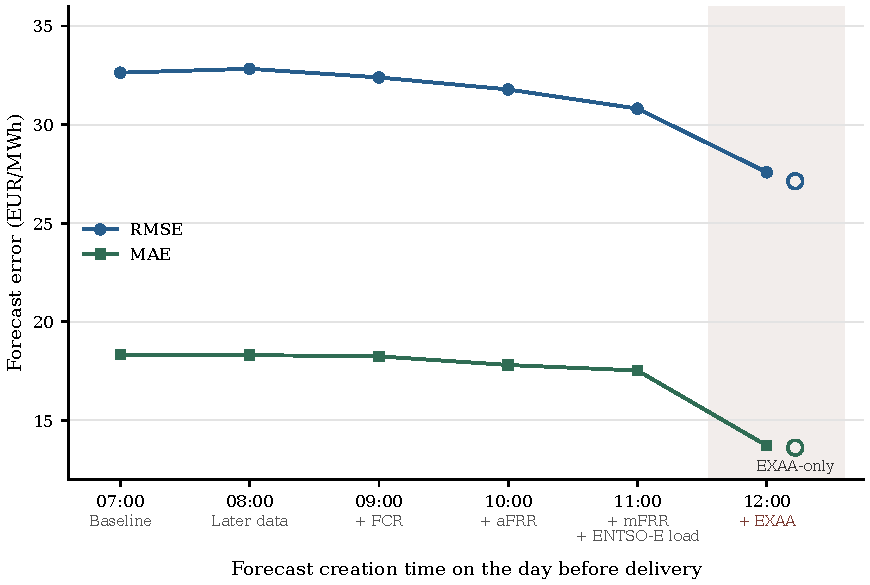
\includegraphics[width=0.78\textwidth]{figures/rq3_cutoff_accuracy.pdf}
  \caption[Price forecast accuracy across forecast creation times.]
  {Price forecast accuracy across the forecast creation times of the cutoff
  grid. The labels below each time name the information added at that cutoff,
  and realized data advance by one hour at every step. The shaded area marks the
  12:00 cutoff, at which EXAA prices become admissible. The hollow markers show
  the compact EXAA-only benchmark.}
  \label{fig:rq3_cutoff_accuracy}
\end{figure}

\FloatBarrier

\hyperlink{hyp:cutoff_sensitivity}{H3} is therefore only partly supported.
Later and richer information sets lower the price forecast error, and the RMSE
at 11:00 is 5.6\% below the 07:00 baseline, but before the EXAA price becomes
available none of these gains is statistically significant. The only significant
improvement, also after the Holm correction, is the step to 12:00. At that
cutoff the EXAA price captures most of the information relevant for the point
forecast, so the compact EXAA-only model matches the full specification, a known
effect for this market rather than a contribution of this thesis.

\FloatBarrier

\subsection{Diagnostic Feature Importance}
\label{sec:results_feature_importance}

The boosted-tree price forecasts are also analyzed with the SHAP values
introduced in Section~\ref{sec:feature_importance}. The forecast experiment
refits a separate LightGBM model for each delivery day on its rolling training
window. For this diagnostic, and for each selected specification, these daily
models are refitted for every delivery day in the evaluation window with the same
training window and hyperparameters, and their SHAP contributions are computed
for all MTUs with LightGBM's built-in TreeSHAP decomposition, then
aggregated by the feature groups defined in Section~\ref{sec:feature_importance}.
Because the price model is fitted on the variance-stabilized target of
Section~\ref{sec:price_model}, the contributions live in that transformed space
and are interpretable in direction and relative magnitude rather than as EUR/MWh
amounts. The grouped shares reported here are unit-free ratios of each group's
contribution to the total, so they are comparable across models but describe
relative importance in the transformed space, not EUR/MWh contributions. They
are diagnostic relative importances within the fitted model, not causal effects.

Figure~\ref{fig:rq2_feature_importance} reports the grouped contribution shares
for the RQ2 price models. In the base model, raw weather and price lags account
for most of the contribution mass, with shares of 43.1\% and 35.4\%, respectively,
and the \mbox{ENTSO-E} load forecast contributes 21.4\%. Once OBTF
forecasts are added, the structure of the model changes: the OBTF
residual-load forecast becomes the most important group, with a contribution
share of 42.3\% against 24.7\% for price lags, while raw weather falls to
13.0\% and the OBTF renewable-generation forecast contributes 15.3\%. In the
weather-free variant, residual load and renewable generation absorb the
weather-driven information directly, at 45.4\% and 21.7\%. This supports the interpretation from RQ2
that the OBTF load and renewable-generation forecasts provide a compact
weather-informed representation of the power-system state.

\begin{figure}[htbp]
  \centering
  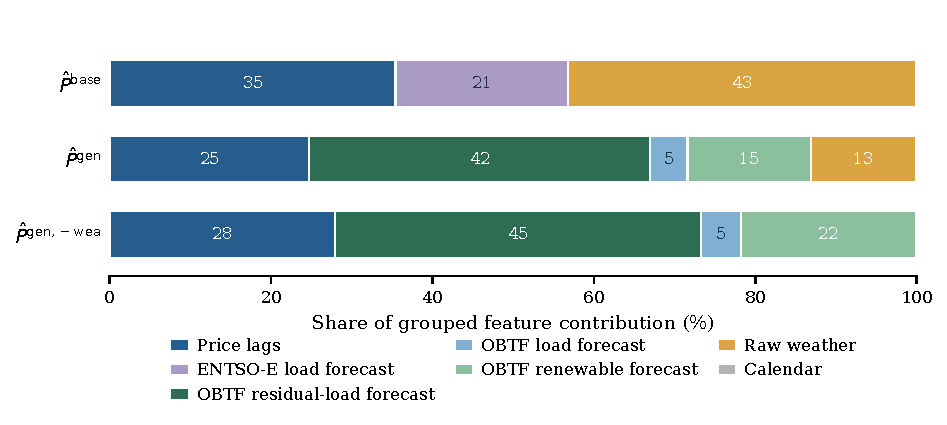
\includegraphics[width=0.86\textwidth]{figures/rq2_feature_importance_bars.pdf}
  \caption[Feature-importance shares for the RQ2 price models.]
  {Grouped feature-contribution shares for the RQ2 price models, as percentages
  of the mean absolute grouped SHAP contribution. The diagnostic covers all delivery days and MTUs in the evaluation window. Shares may not sum exactly to 100 because of
  rounding.}
  \label{fig:rq2_feature_importance}
\end{figure}

Figure~\ref{fig:rq3_feature_importance} reports the same diagnostic for selected
cutoff-grid models. Before EXAA prices become available, the residual-load
forecast and the price lags drive the price forecasts, alongside the renewable-generation
forecast, raw weather, and a growing reserve-market block. The reserve-market
share rises once aFRR information is available, from 4.4\% at 09:00 to 18.5\% at
10:00, and to 20.3\% at 11:00 as mFRR is added. The fitted models therefore make
substantial use of the reserve-market results, even though their contribution to
accuracy is not robustly significant (Section~\ref{sec:results_rq3}). At 12:00,
EXAA prices dominate the feature contributions, at 66.9\% of the mass, although
all other feature blocks are available. Together with the statistically
indistinguishable accuracy of the full 12:00 model and the EXAA-only model, this
is consistent with the late EXAA signal already containing most of the
short-horizon price information that the other feature blocks provide.
Appendix~\ref{app:feature_details} reports the leading subgroups for
\(\hat{P}^{\mathrm{gen}}\) and the 12:00 model, and shows the direction of the
leading effects.

\begin{figure}[htbp]
  \centering
  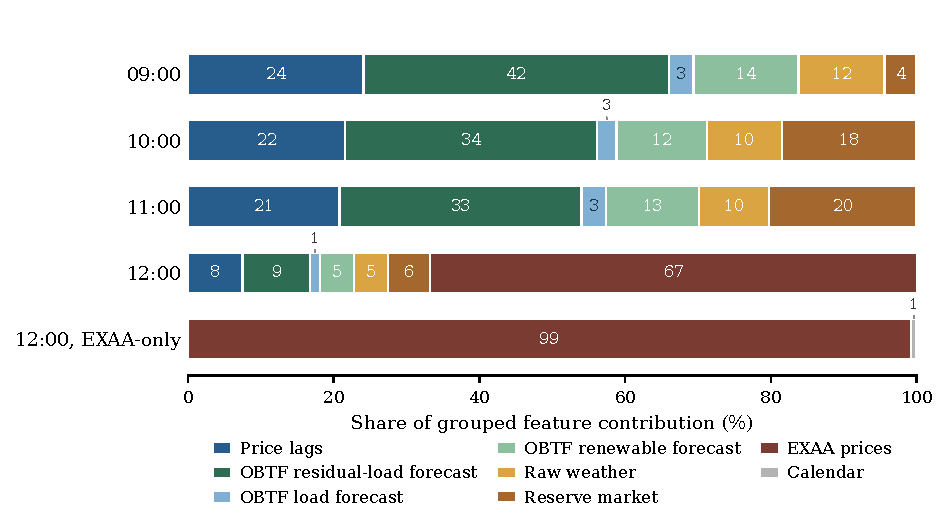
\includegraphics[width=0.86\textwidth]{figures/rq3_feature_importance_bars.pdf}
  \caption[Feature-importance shares for selected RQ3 cutoff models.]
  {Grouped feature-contribution shares for selected RQ3 cutoff models, as
  percentages of the mean absolute grouped SHAP contribution. The calendar group
  is below 1\% throughout. The
  diagnostic covers all delivery days and MTUs in the evaluation
  window. Shares may not sum exactly to 100 because
  of rounding.}
  \label{fig:rq3_feature_importance}
\end{figure}
